% Options for packages loaded elsewhere
% Options for packages loaded elsewhere
\PassOptionsToPackage{unicode}{hyperref}
\PassOptionsToPackage{hyphens}{url}
\PassOptionsToPackage{dvipsnames,svgnames,x11names}{xcolor}
%
\documentclass[
  letterpaper,
]{article}
\usepackage{xcolor}
\usepackage{amsmath,amssymb}
\setcounter{secnumdepth}{-\maxdimen} % remove section numbering
\usepackage{iftex}
\ifPDFTeX
  \usepackage[T1]{fontenc}
  \usepackage[utf8]{inputenc}
  \usepackage{textcomp} % provide euro and other symbols
\else % if luatex or xetex
  \usepackage{unicode-math} % this also loads fontspec
  \defaultfontfeatures{Scale=MatchLowercase}
  \defaultfontfeatures[\rmfamily]{Ligatures=TeX,Scale=1}
\fi
\usepackage{lmodern}
\ifPDFTeX\else
  % xetex/luatex font selection
  \setmainfont[]{Arial}
\fi
% Use upquote if available, for straight quotes in verbatim environments
\IfFileExists{upquote.sty}{\usepackage{upquote}}{}
\IfFileExists{microtype.sty}{% use microtype if available
  \usepackage[]{microtype}
  \UseMicrotypeSet[protrusion]{basicmath} % disable protrusion for tt fonts
}{}
\makeatletter
\@ifundefined{KOMAClassName}{% if non-KOMA class
  \IfFileExists{parskip.sty}{%
    \usepackage{parskip}
  }{% else
    \setlength{\parindent}{0pt}
    \setlength{\parskip}{6pt plus 2pt minus 1pt}}
}{% if KOMA class
  \KOMAoptions{parskip=half}}
\makeatother
% Make \paragraph and \subparagraph free-standing
\makeatletter
\ifx\paragraph\undefined\else
  \let\oldparagraph\paragraph
  \renewcommand{\paragraph}{
    \@ifstar
      \xxxParagraphStar
      \xxxParagraphNoStar
  }
  \newcommand{\xxxParagraphStar}[1]{\oldparagraph*{#1}\mbox{}}
  \newcommand{\xxxParagraphNoStar}[1]{\oldparagraph{#1}\mbox{}}
\fi
\ifx\subparagraph\undefined\else
  \let\oldsubparagraph\subparagraph
  \renewcommand{\subparagraph}{
    \@ifstar
      \xxxSubParagraphStar
      \xxxSubParagraphNoStar
  }
  \newcommand{\xxxSubParagraphStar}[1]{\oldsubparagraph*{#1}\mbox{}}
  \newcommand{\xxxSubParagraphNoStar}[1]{\oldsubparagraph{#1}\mbox{}}
\fi
\makeatother


\usepackage{longtable,booktabs,array}
\usepackage{calc} % for calculating minipage widths
% Correct order of tables after \paragraph or \subparagraph
\usepackage{etoolbox}
\makeatletter
\patchcmd\longtable{\par}{\if@noskipsec\mbox{}\fi\par}{}{}
\makeatother
% Allow footnotes in longtable head/foot
\IfFileExists{footnotehyper.sty}{\usepackage{footnotehyper}}{\usepackage{footnote}}
\makesavenoteenv{longtable}
\usepackage{graphicx}
\makeatletter
\newsavebox\pandoc@box
\newcommand*\pandocbounded[1]{% scales image to fit in text height/width
  \sbox\pandoc@box{#1}%
  \Gscale@div\@tempa{\textheight}{\dimexpr\ht\pandoc@box+\dp\pandoc@box\relax}%
  \Gscale@div\@tempb{\linewidth}{\wd\pandoc@box}%
  \ifdim\@tempb\p@<\@tempa\p@\let\@tempa\@tempb\fi% select the smaller of both
  \ifdim\@tempa\p@<\p@\scalebox{\@tempa}{\usebox\pandoc@box}%
  \else\usebox{\pandoc@box}%
  \fi%
}
% Set default figure placement to htbp
\def\fps@figure{htbp}
\makeatother


% definitions for citeproc citations
\NewDocumentCommand\citeproctext{}{}
\NewDocumentCommand\citeproc{mm}{%
  \begingroup\def\citeproctext{#2}\cite{#1}\endgroup}
\makeatletter
 % allow citations to break across lines
 \let\@cite@ofmt\@firstofone
 % avoid brackets around text for \cite:
 \def\@biblabel#1{}
 \def\@cite#1#2{{#1\if@tempswa , #2\fi}}
\makeatother
\newlength{\cslhangindent}
\setlength{\cslhangindent}{1.5em}
\newlength{\csllabelwidth}
\setlength{\csllabelwidth}{3em}
\newenvironment{CSLReferences}[2] % #1 hanging-indent, #2 entry-spacing
 {\begin{list}{}{%
  \setlength{\itemindent}{0pt}
  \setlength{\leftmargin}{0pt}
  \setlength{\parsep}{0pt}
  % turn on hanging indent if param 1 is 1
  \ifodd #1
   \setlength{\leftmargin}{\cslhangindent}
   \setlength{\itemindent}{-1\cslhangindent}
  \fi
  % set entry spacing
  \setlength{\itemsep}{#2\baselineskip}}}
 {\end{list}}
\usepackage{calc}
\newcommand{\CSLBlock}[1]{\hfill\break\parbox[t]{\linewidth}{\strut\ignorespaces#1\strut}}
\newcommand{\CSLLeftMargin}[1]{\parbox[t]{\csllabelwidth}{\strut#1\strut}}
\newcommand{\CSLRightInline}[1]{\parbox[t]{\linewidth - \csllabelwidth}{\strut#1\strut}}
\newcommand{\CSLIndent}[1]{\hspace{\cslhangindent}#1}



\setlength{\emergencystretch}{3em} % prevent overfull lines

\providecommand{\tightlist}{%
  \setlength{\itemsep}{0pt}\setlength{\parskip}{0pt}}



 


\makeatletter
\@ifpackageloaded{caption}{}{\usepackage{caption}}
\AtBeginDocument{%
\ifdefined\contentsname
  \renewcommand*\contentsname{Table of contents}
\else
  \newcommand\contentsname{Table of contents}
\fi
\ifdefined\listfigurename
  \renewcommand*\listfigurename{List of Figures}
\else
  \newcommand\listfigurename{List of Figures}
\fi
\ifdefined\listtablename
  \renewcommand*\listtablename{List of Tables}
\else
  \newcommand\listtablename{List of Tables}
\fi
\ifdefined\figurename
  \renewcommand*\figurename{Figure}
\else
  \newcommand\figurename{Figure}
\fi
\ifdefined\tablename
  \renewcommand*\tablename{Table}
\else
  \newcommand\tablename{Table}
\fi
}
\@ifpackageloaded{float}{}{\usepackage{float}}
\floatstyle{ruled}
\@ifundefined{c@chapter}{\newfloat{codelisting}{h}{lop}}{\newfloat{codelisting}{h}{lop}[chapter]}
\floatname{codelisting}{Listing}
\newcommand*\listoflistings{\listof{codelisting}{List of Listings}}
\makeatother
\makeatletter
\makeatother
\makeatletter
\@ifpackageloaded{caption}{}{\usepackage{caption}}
\@ifpackageloaded{subcaption}{}{\usepackage{subcaption}}
\makeatother
\makeatletter
\@ifpackageloaded{sidenotes}{}{\usepackage{sidenotes}}
\@ifpackageloaded{marginnote}{}{\usepackage{marginnote}}
\makeatother
\usepackage{bookmark}
\IfFileExists{xurl.sty}{\usepackage{xurl}}{} % add URL line breaks if available
\urlstyle{same}
\hypersetup{
  pdftitle={Advancing Telemedicine in Musculoskeletal Practice},
  pdfauthor={Nathan Cashion},
  pdfkeywords={telemedicine, musculoskeletal, technology, digital
health, academic, thesis},
  colorlinks=true,
  linkcolor={blue},
  filecolor={Maroon},
  citecolor={Blue},
  urlcolor={Blue},
  pdfcreator={LaTeX via pandoc}}


\title{Advancing Telemedicine in Musculoskeletal Practice}
\author{Nathan Cashion}
\date{2024-07-08}
\begin{document}
\maketitle
\begin{abstract}
Telemedicine has rapidly emerged as a promising approach to managing
back, neck, and other musculoskeletal (MSK) pain. Despite impressive
advances in the technology, clinicians and patients remain reluctant to
adopt it. The transition to telemedicine from hands-on, in-person care
presents numerous barriers. In contrast, new technologies and tools are
readily embraced by early-adopters in other industries, such as video
game streaming, fitness influencers, and YouTube content creators. By
adopting tools and techniques from these other industries, MSK providers
may be able to increase in-session engagement and patient satisfaction
with telemedicine.
\end{abstract}

\renewcommand*\contentsname{Table of contents}
{
\hypersetup{linkcolor=}
\setcounter{tocdepth}{3}
\tableofcontents
}

\begin{figure*}

\begin{figure}[H]

{\centering \pandocbounded{\includegraphics[keepaspectratio]{3BroadcastSetup.png}}

}

\caption{\emph{What can telemedicine providers learn from live
streamers?}}

\end{figure}%

\end{figure*}%

\section{Advancing Telemedicine in Musculoskeletal
Practice}\label{advancing-telemedicine-in-musculoskeletal-practice}

Telemedicine has the potential to bring healthcare to millions of
patients who are unable to visit their doctor. This holds true even in
specialties that traditionally demand a face-to-face, such as
chiropractic, osteopathy, physical therapy, and pain medicine.
Surprisingly, these specialties focused on musculoskeletal conditions
have also benefited from the use of telemedicine, particularly during
the COVID-19 pandemic (Lamplot and Taylor 2021).

However, video calls leave much to be wanted, especially for conditions
that are commonly examined and treated with direct, physical touch via
physiotherapy, chiropractic, and massage. Patients and their clinicians
observe feelings of disconnect during their live video calls (Ahmad et
al. 2023). Healthcare systems and private clinics have been slow to
include telemedicine in MSK practice for various reasons, including
cost, resistance to change, and lack of clarity on the benefits and
feasibility in this specialty (Davies et al. 2021). Learning how to make
telemedicine a better experience for both patients and clinicians can
accelerate the potential reach of this promising technology.

\begin{figure*}

\end{figure*}%

\subsubsection{Overview of Topic}\label{overview-of-topic}

\emph{Telemedicine} is defined as the practice of caring for patients
from a distance (Jin et al. 2020). \emph{Telehealth} is a broader term
that can include population-based efforts in public and global health.
In contrast, the focus of telemedicine is on a single patient or small
group of patients (Barberio and Jenkins 2021). \emph{Telerehabilitation}
is another term that is often used interchangeably with telemedicine for
musculoskeletal conditions, particularly physical therapy in
post-surgical scenarios (Baroni et al. 2023). While the topic of this
paper is focused on musculoskeletal applications, most of the concepts
do apply to other specialties. Hence, I will use telemedicine throughout
for consistency.

Telemedicine has been used in various forms for centuries (consider
carrier pigeons being used to suggest tinctures for the plague or phone
calls to the family doctor for a child's late-night stomachache) (Jin et
al. 2020). Modernly, it has become nearly synonymous with
implementations via the internet, such as video conferencing calls
between a provider and a patient (Davies et al. 2021).

Telemedicine offers many benefits to patients, but legislation has not
kept up with demand. As a result of the pandemic, legislation required
insurance companies to pay for telemedicine visits with temporary
exceptions allowing for greater access across state lines (Barberio and
Jenkins 2021). However, while some aspects of this have been extended,
it is unclear whether reimbursement will continue for all services
across all specialties ({``Telehealth Is Here to Stay''} 2021). For
telehealth to have a positive effect on healthcare, several challenges
must be addressed in policy and research.

\subsubsection{Identification of Gap}\label{identification-of-gap}

Beyond the slow adjustments in legislation and reimbursements,
telemedicine has suffered in hasty roll-outs that have not afforded
optimal infrastructure or training to take place. In fact, one of the
key factors in clinicians' reluctance to use telehealth is the lack of
familiarity with the technology and ideal procedures for conducting
virtual visits with patients (Davies et al. 2021).

While most of us were forced to rapidly adapt to a Zoom-centered
culture, using the same tools for different situations can lead to
sub-optimal experiences. A conversation about low back pain, for
example, is meant to be a dynamic collaboration between patient and
provider, often including the use of visuals such as physical anatomical
models to illustrate the underlying structures that may be associated
with pain syndromes. Experiences like these are challenging to achieve
in a 2-dimensional, relatively static video call when both participants
are limited to showing themselves from the mid-torso to above the head.
Even worse, Zoom meetings are often affected by quality issues such as
poor-audio or bad lighting that make it difficult for the participants
to understand one another, let alone forge an emotional connection.
Problems with internet connectivity can interrupt a speaker mid-sentence
or prevent a call from starting altogether.

Advances in audio and video technology, however, make it possible for
amateurs and hobbyists to create high-quality video content, including
well-produced, livestreaming video. Fitness influencers post ultra-high
definition videos to educate and entertain their followers about
healthcare topics on social media and YouTube. From the average bedroom
-- or their parents' basement -- `gamers' broadcast their video game
activities to hundreds of thousands of engaged fans, using tools to
create a dynamic and highly-produced experience that leaves viewers
feeling like they are a part of a community.

Based on my review of the literature, there is little to no discussion
about improving the technical aspects of synchronous telemedicine video
calls and how they influence the patient and clinician experience.
Pulling from the literature on user experience design, live video
streaming, and incorporating skills from audio and video engineering, it
is possible to greatly improve the experience and satisfaction of all
involved.

\subsection{Background}\label{background}

\subsubsection{Selection of Topic}\label{selection-of-topic}

As a chiropractor with a passion for technology, I have been fascinated
by the possibilities of providing spine care remotely, both via
telemedicine or asynchronous media such as mobile apps and tools using
artificial intelligence. Spurred on by the COVID-19 pandemic,
telemedicine has become more common throughout all specialties,
including for musculoskeletal conditions normally treated by
chiropractors and physiotherapists (Lamplot and Taylor 2021). However,
due to the hands-on nature of manual therapy offered as treatment for
musculoskeletal aches and pains, patients and providers have expressed
doubts as to the practicality of telemedicine (Barton et al. 2022).
While physical therapies are prominent, other components of
evidence-based musculoskeletal care include education and exercise
prescription, both of which can be provided effectively via telemedicine
solutions (Baroni et al. 2023).

Patients who opt for telemedicine visits have reported positive
outcomes, even if they were initially skeptical (Rana S. Hinman et al.
2024; Lawford et al. 2018). According to Ernstzen et al. (2022),
patients experiencing chronic pain who joined a group exercise program
found that it helped them feel empowered. Multiple studies have
determined that for patients with musculoskeletal disorders,
telemedicine is as safe and effective as in-person care (Bargeri et al.
2024; Seron et al. 2021; Withers et al. 2024).

Despite this early success, many barriers still exist that prevent more
widespread adoption of telemedicine. Using a qualitative approach, Wade,
Eliott, and Hiller (2014) concluded that clinician acceptance is the
leading factor limiting adoption of telemedicine, followed by patient
acceptance. This reluctance is reflected in the previous findings that
remotely delivered care does not meet the patient's expectation of
hands-on touch (Baroni et al. 2023). Saragiotto, Sandal, and Hartvigsen
(2022) commented on this paradox of being a manual therapist but not
using your hands. While they found the existing literature on
telemedicine was limited, the available evidence suggests that
practitioners of manual therapies are able to have a positive effect on
reducing pain and improving function in patients with musculoskeletal
conditions in a virtual setting. Therefore, the authors recommended that
manual therapists include telemedicine in their available options for
treatment.

Other criteria for resistance to telemedicine include a lack of
familiarity with the technology, referred to as \emph{digital literacy}
(Fernandes and Saragiotto 2021; Manganello et al. 2017), and the ability
to build rapport and develop a therapeutic alliance between patient and
practitioner (Wallace et al. 2022).

This final point has captured my attention and imagination. What is it
about the experience on video calls that has people feeling
disconnected? What are the elements that lead to the so-called ``Zoom
fatigue'' so many of us have experienced during the rapid shift to
virtual communication during the pandemic (Bailenson 2021)? Are there
solutions that are already being used in other industries to increase
the feeling of connectedness and engagement during telemedicine
appointments?

Most research to date has evaluated the presence of telemedicine in care
settings as well as the results in terms of patient outcomes and safety.
But have researchers considered that \emph{how} telemedicine visits are
conducted may have an impact on the outcomes? In most other areas of
technology, immense effort and millions of dollars are spent on refining
the user-experience (UX) of digital tools and software to increase user
satisfaction (Monachelli et al. 2024). What changes could be made to the
UX of telemedicine to increase patient satisfaction and decrease
clinician burden?

\subsubsection{Literature Search}\label{literature-search}

I conducted a series of searches using EBSCOHost. A broad search for
\texttt{"telehealth"} returned 180,725 results. Adding the terms
\texttt{"telemedicine\ OR\ telehealth\ OR\ telerehab*"} reduced my
results to 800+. I further limited the search to relevant papers using
the term \texttt{"musculoskeletal"}. As technology is a rapidly
advancing field, I limited the Publication Date to between 2019-2024.
Source types were restricted to Academic Journals and Reviews.

Searches for \texttt{"telehealth\ AND\ engagement"} provided limited
results relevant to the current topic. I conducted further searches via
PubMed on engagement in live streaming applications, such as video games
and ecommerce with the terms
\texttt{"live\ streaming\ AND\ engagement"}. Results were varied and I
narrowed the selection by scanning titles and abstracts for relevance,
then reviewing related papers and papers cited by or citing the current
paper.

I included other articles found via Google Scholar and Google Search
that were relevant. Though they may not be peer-reviewed, they are
authored by industry experts.

When new topics or keywords appeared frequently in my initial results, I
explored them further by searching the same databases. I also used
artificial intelligence research assistants (Elicit 2024; Research
Rabbit 2024) to suggest other articles or related topics.

\subsubsection{Literature Review}\label{literature-review}

My literature brought together research in two broad areas---the use of
telemedicine in musculoskeletal health and the psychology of engagement
in live-streaming video.

A review of the existing literature on telemedicine in musculoskeletal
care revealed a number of themes. The majority of the research addressed
trends in the use of telemedicine broadly. This thread of the literature
included prevalence of remote therapies as well as acceptance and
perceptions by both clinicians and patients. The second most common
theme in the research concerned the reliability of the examination and
diagnosis of musculoskeletal disorders via telemedicine as well as the
effectiveness of treatment. Other themes included the core competencies
suggested for clinicians to conduct telemedicine visits and the
limitations of telemedicine in practice.

\paragraph{Telemedicine in MSK care}\label{telemedicine-in-msk-care}

\emph{Trends in use and acceptance of telemedicine}

Out of necessity, the use of telemedicine accelerated during the global
COVID pandemic. A Nature Medicine editorial reflects on the trajectory
of telehealth during the COVID-19 pandemic ({``Telehealth Is Here to
Stay''} 2021). According to Medicare data, telehealth visits increased
ten-fold in a 12-month period (from March 2020--March 2021).

Telemedicine is not only used for individuals. Several programs have
explored adapting group programs for chronic pain to a virtual setting.
Wallace et al. (2022) conducted a scoping review of group and individual
telehealth for chronic musculoskeletal pain to explore patient
perspectives on virtually delivered pain management programmes. From 10
included studies, the authors extracted 4 themes: usability of the
technology, tailored care, therapeutic alliance, and managing behavior.
The authors determined that telehealth for chronic musculoskeletal pain
is acceptable by patients. Group telehealth programs additionally offer
opportunities for social support and validation of the pain experience.
Patients felt empowered and intrinsically motivated to modify their
behaviour. The authors discussed how clinicians can help develop a
therapeutic alliance during telehealth interventions. This is more
readily accomplished via synchronous video-conferencing rather than
asynchronous messaging.

South Africa offers a group Patient Education Empowerment Programme
(PEEP) for patients living with chronic pain. Due to the pandemic, this
program was adapted to be delivered remotely via synchronous (group
calls) and asynchronous (educational materials) methods. Ernstzen et al.
(2022) interviewed six women who participated in this 6-week telehealth
group program to learn what worked and what didn't. The patients felt
that the program helped them start on a journey of self-discovery and
personal development. Connecting with other patients experiencing
similar pain and disability helped validate their experiences and
motivated them to alter their behaviors. Participants reported that this
method of delivering a group program for chronic musculoskeletal pain
was feasible and that they felt engaged and supported. Facilitators were
able to develop a therapeutic alliance through virtual communication
without meeting patients in person. While there were barriers to
comfortably participating in this course, facilitators were able to
address them with planning. For example, data packages were provided to
patients to cover the cost of increased cellular data usage.

Ahmad et al. (2023) surveyed nearly 500 patients who had received
telemedicine care for hand surgery consultation during the pandemic. The
majority of respondents liked their experience of a teleconsultation and
felt satisfied with the attention recieved from their provider. Despite
this, over two-thirds of the patients said they would still prefer an
in-person visits when available. Common reasons for this choice included
difficulty explaining their symptoms and the need for an in-person
follow-up visit to move forward with their care.

\emph{Diagnosis and management of MSK conditions via telemedicine}

Oh et al. (2024) reviewed 9 studies on the assessment and management of
people with MSK conditions. They found that inter-rater reliability for
diagnosis involving the low back, knee, shoulder, lower limb, ankle,
elbow, and shoulder was high. The authors concluded that telehealth is a
feasible option for assessment of musculoskeletal conditions.

Satin and Lieberman (2021) provided a narrative review on how clinicians
can conduct physical examination for spine-related disorders via virtual
calls. The authors presented strategies for overcoming some of the
difficulties unique to virtual examination of the spine.

A systematic review from Bernhardsson et al. (2023), compared
face-to-face physiotherapy assessment of musculoskeletal disorders with
convential assessment. Digital physiotherapy assessment was found to
have moderate to almost perfect validity when compared to traditional
physical exams. The authors explained that while patients thought an
in-person assessment was better, they were satisfied with their
experience. The reported outcomes also demonstrated excellent
reliability of patient-reported outcome measures.

A study in India showed that telerehabilitation for spine pain reduced
pain and disability better than standard in-clinic rehabilitation during
the COVID pandemic (Shah et al. 2024). As reported by Barberio and
Jenkins (2021), an overview of clinical outcomes and patient
satisfaction concluded that telemedicine offered equal or better results
than usual care.

\emph{Core competencies for telemedicine in MSK}

Davies et al. (2021) conducted a modified Delphi survey ith experts in
physiotherapy, including researchers, clinicians, consumers, and
representatives of physiotherapy organizations. The panel developed a
framework to outline the skills and capabilities needed to deliver care
via video calls. The recommendations consisted of legal and ethical
topics such as patient privacy \& safety, record keeping, and licensure.
The panel also outlined technical skills such as camera placement,
software selection, and adapting the physical exam to a virtual setting.

Haldeman et al. (2021) describe the process of developing a pair of
guides to help clinicians and patients manage spinal pain during the
COVID-19 pandemic or in any situation that requires management from a
distance. A group of 29 individuals from 10 countries including
experienced clinicians, researchers, and educators collaborated through
an iterative process to create two guides. The Patient Guide includes 2
steps to help patients self-assess the severity and nature of their
spinal pain and determine an appropriate course of action, such as
emergency care, urgent care, or non-urgent communication with a
healthcare provider. The Clinician Guide provides a framework for
providers to systematically assess and classify patient's spinal
disorders. The authors suggest that telehealth visits will provide a
helpful method for patients and clinicians to evaluate and manage spinal
disorders when face-to-face visits are not available.

\emph{Limitations of telemedicine}

As telehealth becomes more popular and widespread, it is important to
recognize the strengths and weaknesses of this new platform. While many
clinicians and patients see the lack of hands-on care as a drawback
(Barton et al. 2022), manual therapy is just one of many modalities that
clinicians can use to manage patients with musculoskeletal conditions.
Nevertheless, while physical touch isn't required in medicine, it is
still appropriate to consider the inherent value in skin-to-skin
contact.

Apathy et al. (2024) recognize that providers offering telemedicine must
change their workflow. The authors analyzed how much time clinicians in
a large multispecialty clinic spent on their EHR in two types of visits
-- telemedicine and standard, in-person visits. The goal was to identify
whether offering telemedicine visits changed the amount of time spent on
EHR documentation.

The authors found that on days with telemedicine visits, clinicians
spent an average of 14.8 minutes more on documentation in the EHR
compared to days with no telemedicine visits. However, on days with only
telemedicine visits, there was no increase in time spent in the EHR.
This suggests that mixing in-person and telemedicine visits in the
clinic may lead to inefficiencies as opposed to dedicating certain days
to telemedicine visits. This suggests that a hybrid approach has
drawbacks. If clinicians dedicate time to telemedicine, they may see
improved outcomes.

\paragraph{Engagement in a virtual
setting}\label{engagement-in-a-virtual-setting}

Most of the research concerning engagement in telemedicine refers to the
long-term involvement of patients in their own care (Lyles et al. 2020;
Monachelli et al. 2024). Little research has evaluated the ways in which
telemedicine providers can increase real-time engagement and
satisfaction of their patients during synchronous calls. However,
relevant literature exists in other applications of virtual live
streaming such as e-commerce and gaming. The second part of my
literature review addressed research exploring engagement and feelings
of connection between live-streamers and their audience.

\emph{Application of intimacy theory}

Liu, Sun, and Lee (2021) examined viewer engagement in ecommerce
streaming, where a presenter reviews or discusses products with a goal
to sell to their audience. The authors promote \emph{intimacy
theory}---the idea that acting in an authentic and transparent manner
builds trust and intimacy---as a model for engaging live viewers.
Several suggestions are offered. Live streamers should: - respond
quickly to viewers comments or questions - present a consistent and
authentic personal brand - demonstrate attudinal similarity by mirroring
viewer's beliefs or opinions - speak directly to viewers - simulate
direct eye contact by looking directly into the camera.

Baroni et al. (2023) emphasized this last point stating that
communication is the most powerful tool for clinicians to use in
telemedicine consults. Looking directly into the camera helps establish
an emotional connection and build trust.

\begin{figure}[H]

{\centering \pandocbounded{
\includegraphics[keepaspectratio]{slide-10.png}}

}

\caption{\emph{Looking directly into the camera can simulate eye contact
and help build professional intimacy.}}

\end{figure}%

Lv et al. (2022) examined factors that lead to sustained engagement by
viewers of live streaming media. The authors hypothesized that there is
a link between visual stimuli (such as emojis), perceived trust, and
presenter's social warmth and continued viewing. The authors developed a
questionnaire that received 240 responses to validate their hypotheses.
Based on their findings, the authors recommend live-streaming presenters
engage their audience in real-time and build long-term trust by
answering questions, designing visual stimuli to support engagement, and
demonstrating social warmth.

\begin{figure}[H]

{\centering \pandocbounded{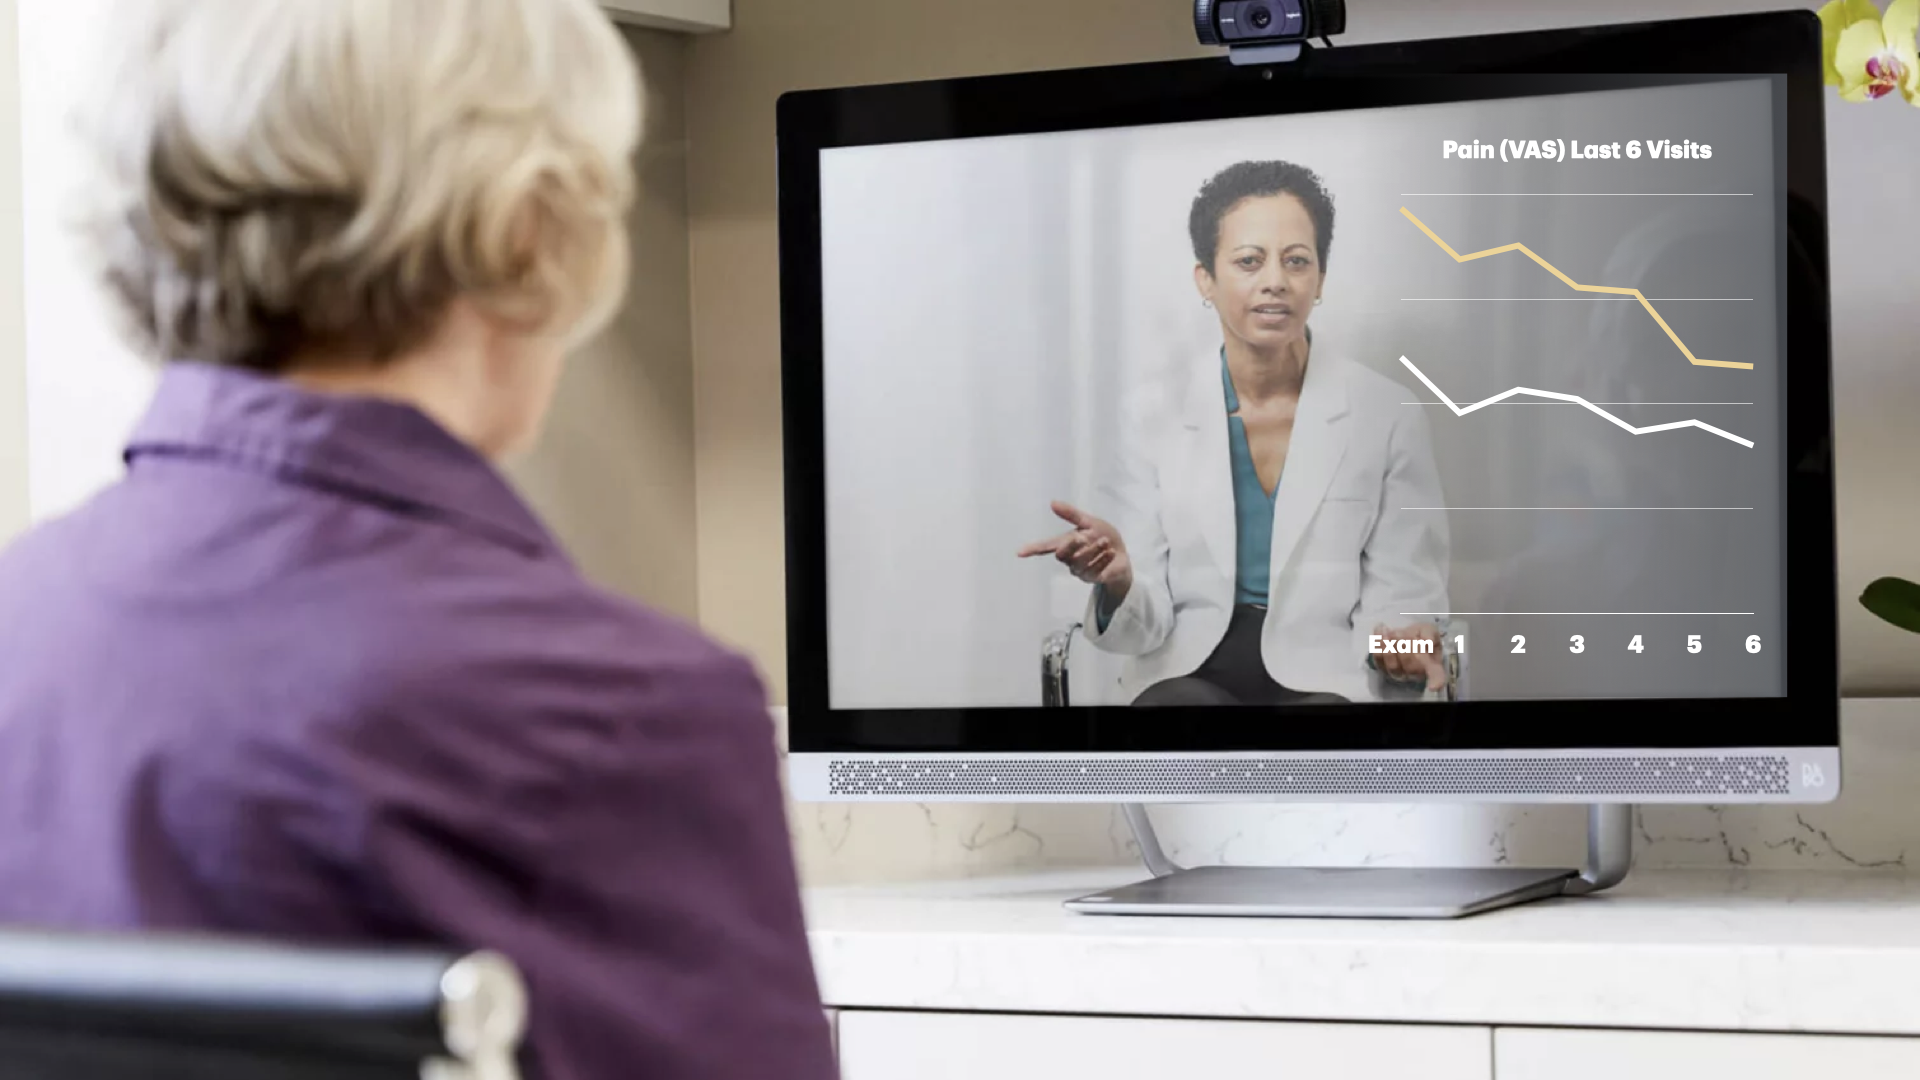
\includegraphics[keepaspectratio]{TelehealthOverlayConcept.002.png}}

}

\caption{\emph{By incorporating visual stimuli, telemedicine providers
can increase patient engagement.}}

\end{figure}%

In their JAMA viewpoint, Mangione, Basile, and Post (2024) reflect on
the power of touch that has become increasingly absent in medicine.
Amongst the various empirical benefits such as improved immune response,
lower blood pressure, oxytocin and endorphin release, the author
highlights the simple recognition that patients appreciate touch.
Mangione observes that along with physical touch, eye contact has also
decreased in the exam room (this is not a necessary casualty of
telehealth---providers can simulate eye contact by learning to look
directly into the camera).

\emph{Content quality}

Li et al. (2023) examined how the characteristics of fitness influencers
impacted people's perceived connection and behaviors. The authors found
that personal attributes, such as attractiveness, and the quality of
content were associated with viewers' motivations to exercise. By
presenting high quality content and engaging with their viewers, social
media influencers facilitated parasocial relationships which positively
influence their viewers' behaviors. This research suggests that content
quality is an important factor in achieving desired results from
viewers.

\begin{figure}[H]

{\centering \pandocbounded{\includegraphics[keepaspectratio]{3CleoAbram.png}}

}

\caption{\emph{YouTubers like Cleo Abram focus on content quality over
quantity, resulting in high viewer engagement.}}

\end{figure}%

\subsection{Problem}\label{problem}

Most of us were forced to get comfortable with remote work and virtual
conferencing during the pandemic. After an initial learning curve,
people began recognizing the myriad benefits of not having to go into
the office such as avoiding traffic, increased productivity, and the
convenience of flexible schedules (Molla 2022; Tsipursky 2023). But as
more time passed, those benefits lost their novelty and people began
noticing negative effects, often referred to as \emph{Zoom fatigue}
(Bailenson 2021). Many companies made the controversial call to return
to the office.

A similar pattern is emerging with the prevalence of telemedicine
visits. According to data from the National Center for Health
Statistics, the percentage of people who used telemedicine visits
declined by 7\% from 2021 to 2022, after a dramatic rise in the early
pandemic (Lucas and Wang 2024).

But what if these negative effects of remote work and video conferencing
were not inherent to the tools, but attributable to user error? Lindsay
(2021), an expert in live streaming media, discussed the common
perception of Zoom fatigue and why he considers it a misconception. He
argues that by learning some basic skills familiar to those in the
broadcast industry, online conferencing does not necessarily lead to
disconnect. Rather, by embracing a virtual-first approach and acquiring
readily available tools, connecting over video-conferencing can actually
feel more authentic and personal. A similar mechanism may explain the
subpar experience as the world has transitioned to more frequent
telemedicine video calls.

Lindsay (2019), also reflects on another technology transition to
illustrate the current limitations in video broadcasting. When motion
pictures were first produced in theaters, they were essentially films of
stage plays. Over the decades, filmmakers realized they were not
constrained by the physical stage and began using different techniques
to push the technology further. Cinema today looks nothing like those
first motion pictures, which Lindsay calls quaint. Similarly, conducting
telemedicine visits in the same way we take business calls over Zoom is
quaint. There is so much more the technology can offer us and we don't
need to be constrained by old formats.

For most providers, telemedicine is a secondary option -- a backup for
when an in-person visit is unavailable or the patient is too far away.
They try to do everything they would in a normal visit, but confine
themselves to a laptop screen and standard Zoom call. If they're feeling
adventurous, they might try a screenshare, but usually they'll just talk
while looking at the patient's chart in an EMR next to -- or even in
front of -- the video window.

This approach might work fine for some specialties. Routine visits with
a primary care provider to review lab results, for example, or a 6 month
post-op check-in with a surgeoun don't require much more than a chat.
But other specialties that involve a more hands-on approach and the need
to see whole-body movement leave a lot to be desired (Barton et al.
2022).

What if we could rethink the virtual visit and re-imagine it with fresh
eyes? Instead of simply inserting the Zoom window into an existing
clinical workflow, what if we built a new encounter around the tools
currently available for connecting with people from afar?

Companies are attempting to create advanced methods of providing
telemedicine such as the Holobox which recreates a full-body 3D
projection of the caller ({``Telehealth with {Holograms}''} 2023). But
these solutions are impractical and out of reach for the average
clinician and patient at the present moment. Other innovators are
turning to virtual reality headsets, like the Apple Vision Pro (Sisson
2024). But these devices are still clunky and create a completely
different paradigm than what patients and providers are used to.

Another approach to managing musculoskeletal conditions from a distance
involves removing the clinician from the synchronous interaction. Wei,
McElroy, and Dey (2019) proposed a novel virtual physical therapist
system for patients with Parkinson's disease. By using Microsoft Kinect
sensors and machine learning algorithms, rehabilitation exercises can be
monitored and adjusted by an application with occasional review by a
physical therapist. In a similar way, Sword Health, a digital physical
therapy provider, provides AI-augmented care plans and motion sensors to
treat musculoskeletal (MSK) conditions (Herzlinger and Lobb 2022). While
such innovations are promising, they are so far outside of the current
healthcare delivery paradigm that they are unlikely to be readily
adopted by current healthcare systems.

These initiatives demonstrate, however, that to make progress in
healthcare, it is often helpful to look to outsiders who can reframe the
problem (Khosla Ventures 2023; Staeritz 2021). Let's look to another
industry that has made live, synchronous video engaging and popular --
video game streaming.

Gamers use off-the shelf video and audio gear together with free,
open-source software to produce high-definition, engaging live-streams
from their bedroom. According to StreamYard ({``How {Much Money Do
Twitch Streamers Make} in 2023?''} 2023), these productions draw
millions of viewers and earn top streamers a healthy six-figure monthly
income. This prompts the question:

\paragraph{\texorpdfstring{\textbf{What can telemedicine providers learn
from live
streamers?}}{What can telemedicine providers learn from live streamers?}}\label{what-can-telemedicine-providers-learn-from-live-streamers}

The current research on telemedicine shows it is a viable alternative
for most of what occurs during regular visits. Gathering the patient's
subjective complaints, conducting a history, performing a comprehensive
exam, determining a likely diagnosis and prognosis, and providing
patient education can all be done as well or better than in-person for
many conditions, including spine pain (Ansary, Martinez, and Scott 2021;
Satin and Lieberman 2021).

Qualitative research on telemedicine offerings reveal generally positive
feedback from patients and clinicans with the occasional mention of
barriers to access or problems with connection (R. S. Hinman et al.
2017; Ahmad et al. 2023). More guidelines are offering suggestions for
including telemedicine in medical education curriculum (Davies et al.
2021). However, these consensuses are limited to basic concepts of
patient safety, privacy, and basic digital literacy -- all important,
but insufficient to make significant improvements beyond the status quo.

\subsection{Plan}\label{plan}

Telemedicine has proven to be a valuable component to evidence-based
musculoskeletal care. However, barriers exist that limit the reach of
this valuable tool. By addressing the perception that telemedicine is
inferior to in-person visits as well as the real-time experience during
video calls, this research may help to persuade more providers to adopt
telemedicine as a viable means to providing education and guidance to
people in pain.

In addition to training musculoskeletal clinicians on core competencies
related to telemedicine, additional training should be offered on
advanced topics, such as intimacy theory to develop a strong therapeutic
alliance and the software and tools to enhance the user-experience.

The group fitness app Peloton is an example of what well-produced
telemedicine can aspire to. Professional instructors guide a live or
virtual group of cyclists through a pre-planned workout that is
broadcast to subscribers. A small technical crew operate the studio and
use multiple camera angles to create a dynamic, choreographed
performance. The instructor is trained to speak directly to an imagined
participant while looking into the camera. This significant effort
results in a unique, engaging experience that journalists have described
as intimate, citing social media posts idolizing the celebrity
instructors (Bryant 2020).

\begin{figure}[H]

{\centering \pandocbounded{\includegraphics[keepaspectratio]{PelotonWideRightShot.png}}

}

\caption{\emph{Peloton instructors are trained to speak directly to
participants while taking advantage of multiple camera angles.}}

\end{figure}%

While Peloton is a high-end luxury fitness brand, there are elements to
the production that can be applied to telemedicine. Clinicians can be
trained to build a stronger connection with their patients over video
calls by incorporating the elements of authenticity and looking directly
into the camera. Using additional software and hardware, clinicians can
choose from different camera angles that allow them to demonstrate
full-body movements with side- or front-views as well as returning to a
standard, close-up view when listening to or speaking to the patient.
This software can also be configured to seamlessly show additional
content such as radiographs that can be annotated in real-time or
data-visualizations showing the patient's progress with treatment.

Virtual webcam software is one option to enhance the telemedicine
experience. Open Broadcaster Software (OBS) is a free and open-source
cross-platform application built for video live streaming ({``Open
{Broadcaster Software}''} n.d.). eCamm Live is a commercial alternative
that offers a shorter learning curve and more refined user-interface,
but is only available for macOS ({``Ecamm {Live}''} n.d.). Both
applications have a similar feature set, including the ability to build
custom `scenes' with a particular layout of video, audio, and screen
sources. The operator (in this case a telemedicine provider) can switch
between these scenes on the fly with the push of a button. For example,
a provider can start with a simple close-up angle to open the call,
switch to a full-body angle while demonstrating clinical exam
procedures, then switch to a scene with both close-up video and a window
capture showing a digital anatomical model of a body part of interest.

Another popular tool in live streaming is the Elgato StreamDeck, a small
keypad with customizeable buttons and software that integrates with
various applications including OBS and eCamm Live ({``Stream {Deck
MK}.2''} n.d.). The StreamDeck can act as a hardware controller for OBS
or eCamm to switch between scenes or trigger animations or other actions
on the video call. Elgato also makes the Prompter, a small display with
a one-way mirror that acts as a teleprompter. This---or other
teleprompter devices---can be used to place the incoming video of a
patient directly in front of the camera lens, making it easy for the
provider to maintain eye contact throughout the call.

Combining these tools with a variety of options for additional cameras,
lighting, and audio equipment can allow a provider to create a powerful
telemedicine studio. Paired with clinician training to take advantage of
these new tools and engage the patient effectively, this set-up can
enhance the quality of telemedicine video calls.

\subsubsection{Key Uncertainties}\label{key-uncertainties}

Despite the promising potential of this proposal, a few areas of
uncertainty remain.

\emph{Security and Confidentiality}

As previously mentioned, patient privacy and confidentiality are key
concerns in healthcare, including in telemedicine. Clinical software is
required to by HIPAA compliant and is often reviewed by the Federal Drug
Administration (Jin et al. 2020). Programs such as OBS and eCamm Live
are designed to be used in one-to-many live-streaming scenarios, which
may not involve the end-to-end encryption now required of telehealth
platforms. However, this broadcast function is not on by default. The
app simply inserts itself in the video pipeline to act as a virtual
webcam, and all processing of the video and audio data is done
on-device. The software can work with HIPAA-compliant telehealth
software such as Zoom or Doxy.me. Nevertheless, the open-source nature
of these tools raises concerns about HIPAA-compliance and security that
must be addressed before these recommendations are implemented.

\emph{Financial and Logistic Feasibility}

Compared to professional broadcast gear, the software and devices
discussed are accessible and inexpensive. Yet, they do constitute an
additional expense beyond the current standard set-up for
musculoskeletal telemedicine providers. The increased cost includes
hardware (additional cameras, microphone, lighting, StreamDeck, etc.)
and potential licensing or subscription fees for virtual webcam
software. This cost can be mitigated by the use of open source software
which does not require any licensing or subscription fees.

Additional expenses will be incurred to develop and deliver training for
musculoskeletal providers. Budgets should account for time in training
sessions and additional support staff to assist with the transition. Due
to the uncertain regulations around reimbursements for virtual care,
clinics and healthcare systems may find it difficult to justify these
additional expenses. Private clinics or individual providers who are
able to make telemedicine a dedicated offering may have a better
business case for adopting this approach.

\emph{Dedicated space}

Another challenge to this proposal will be finding the physical space
necessary to create the appropriate environment. A dedicated
telemedicine studio would be an ideal scenario. The space should allow
for the clinician to move in three dimensions with enough distance to
the camera that their whole body can be visible when needed. A 60 square
foot space with a minimum length of 6 feet in any one direction should
be sufficient. However, in current practice many clinicians conduct
telemedicine calls in a small office space shared with other providers
or used as storage for medical equipment or medical records.

Additionally, a properly prepared space will take acoustics into
account. The feeling of safety in telehealth is important. As a patient
receiving mental health care via a telemedicine platform, I found it
very difficult to be open and unguarded during video call telehealth
sessions. The presence of other voices in my therapist's home office
made me concerned that they could also hear me, which hindered my
ability to speak openly. This experience highlights the significance of
properly treating a room for audio in telehealth settings. It is not
only about preventing sound from going out but also about preventing
sound from coming in. This is crucial in gaining users' trust and
creating a secure environment for open communication. This constitutes
an additional expense and expertise to complete the modifications.

\emph{Increased inequity}

Health inequality is an important issue in healthcare, particularly
among people in low- and middle-income countries. Unfortunately, the
very nature of digital health tools excludes a significant portion of
the popultation who most need access to care. The World Health
Organization reports that one third of the global population are in need
of rehabilitation services (Gimigliano and Negrini 2017). The majority
of these individuals live in areas with lower healthcare resources. They
also lack the health and digital literacy needed to be able to
participate in telemedicine activities (Fernandes and Saragiotto 2021).

The economic and social barriers to telemedicine are difficult to
address. And my proposal is not a solution to them. In fact, in the
beginning it may actually lead to greater disparity, unfortunately.
There is increased cost and necessary training on the part of providers.
But my hope is that by pushing the technology forward and making it more
effective now, it will be easier to bring it to a wider audience in the
near future.

\subsection{Recommendations}\label{recommendations}

To improve the provision of telemedicine, research and training
initiatives should address new ways of conducting virtual visits and
advancing the technical skills of clinicians beyond the core
competencies and basic digital skills. By adopting technical tools from
video production, broadcast, and livestreaming, providers can increase
the quality of their video calls and more readily adapt to the unique
needs of musculoskeletal care. By training clinicians how to foster
emotional connection with enhanced communication skills and maintaining
eye contact during calls, it may be possible to improve the patient
experience, increase satisfaction, and affect outcomes.

\subsubsection*{References}\label{references}
\addcontentsline{toc}{subsubsection}{References}

\phantomsection\label{refs}
\begin{CSLReferences}{1}{0}
\bibitem[\citeproctext]{ref-ahmadPatientPerspectivesTelemedicine2023}
Ahmad, Farhan, Robert W. Wysocki, John J. Fernandez, Mark S. Cohen, and
Xavier C. Simcock. 2023. {``Patient {Perspectives} on {Telemedicine
During} the {COVID-19 Pandemic}.''} \emph{HAND} 18 (3): 522--26.
\url{https://doi.org/10.1177/15589447211030692}.

\bibitem[\citeproctext]{ref-ansaryVirtualPhysicalExam2021}
Ansary, Ali M, Joseph N Martinez, and John D Scott. 2021. {``The Virtual
Physical Exam in the 21st Century.''} \emph{Journal of Telemedicine and
Telecare} 27 (6): 382--92.
\url{https://doi.org/10.1177/1357633X19878330}.

\bibitem[\citeproctext]{ref-apathyTelemedicineInPersonVisit2024}
Apathy, Nate C., Garrett Zabala, Kylie Gomes, Patti Spaar, Seth A.
Krevat, and Raj M. Ratwani. 2024. {``Telemedicine and {In-Person Visit
Modality Mix} and {Electronic Health Record Use} in {Primary Care}.''}
\emph{JAMA Network Open} 7 (4): e248060.
\url{https://doi.org/10.1001/jamanetworkopen.2024.8060}.

\bibitem[\citeproctext]{ref-bailensonNonverbalOverloadTheoretical2021}
Bailenson, Jeremy N. 2021. {``Nonverbal Overload: {A} Theoretical
Argument for the Causes of Zoom Fatigue.''} \emph{Technology, Mind, and
Behavior} 2 (1). \url{https://doi.org/10.1037/tmb0000030}.

\bibitem[\citeproctext]{ref-barberioTransitioningTelehealthTodays2021}
Barberio, Judith Ann, and Melinda L. Jenkins. 2021. {``Transitioning to
{Telehealth}: {Today}'s {Guidelines} for {Future Sustainability}.''}
\emph{The Journal for Nurse Practitioners} 17 (7): 795--98.
\url{https://doi.org/10.1016/j.nurpra.2021.04.001}.

\bibitem[\citeproctext]{ref-bargeriEffectivenessTelemedicineMusculoskeletal2024}
Bargeri, Silvia, Greta Castellini, Jacopo Antonino Vitale, Stefania
Guida, Giuseppe Banfi, Silvia Gianola, and Federico Pennestrì. 2024.
{``Effectiveness of {Telemedicine} for {Musculoskeletal Disorders}:
{Umbrella Review}.''} \emph{Journal of Medical Internet Research} 26
(1): e50090. \url{https://doi.org/10.2196/50090}.

\bibitem[\citeproctext]{ref-baroniStateArtTelerehabilitation2023}
Baroni, Marina P., Maria Fernanda A. Jacob, Wesley R. Rios, Junior V.
Fandim, Lívia G. Fernandes, Pedro I. Chaves, Iuri Fioratti, and Bruno T.
Saragiotto. 2023. {``The State of the Art in Telerehabilitation for
Musculoskeletal Conditions.''} \emph{Archives of Physiotherapy} 13 (1):
1. \url{https://doi.org/10.1186/s40945-022-00155-0}.

\bibitem[\citeproctext]{ref-bartonItsSecondBest2022}
Barton, C. J., A. M. Ezzat, M. Merolli, C. M. Williams, T. Haines, N.
Mehta, and P. Malliaras. 2022. {``{`{It}'s Second Best'}: {A}
Mixed-Methods Evaluation of the Experiences and Attitudes of People with
Musculoskeletal Pain Towards Physiotherapist Delivered Telehealth During
the {COVID-19} Pandemic.''} \emph{Musculoskeletal Science \& Practice}
58 (April): 102500. \url{https://doi.org/10.1016/j.msksp.2021.102500}.

\bibitem[\citeproctext]{ref-bernhardssonDigitalPhysiotherapyAssessment2023}
Bernhardsson, Susanne, Anette Larsson, Anna Bergenheim, Chan-Mei
Ho-Henriksson, Annika Ekhammar, Elvira Lange, Maria E. H. Larsson, Lena
Nordeman, Karin S. Samsson, and Lena Bornhöft. 2023. {``Digital
Physiotherapy Assessment Vs Conventional Face-to-Face Physiotherapy
Assessment of Patients with Musculoskeletal Disorders: {A} Systematic
Review.''} \emph{PLOS ONE} 18 (3): e0283013.
\url{https://doi.org/10.1371/journal.pone.0283013}.

\bibitem[\citeproctext]{ref-bryantTheresIntimacyWhat2020}
Bryant, Kenzie. 2020. {``{`{There}'s an {Intimacy} to {What We Do}'}:
{How Peloton Became Must-Watch TV} in 2020.''} \emph{Vanity Fair},
December.

\bibitem[\citeproctext]{ref-daviesInternationalCoreCapability2021}
Davies, Luke, Rana S Hinman, Trevor Russell, Belinda Lawford, Kim
Bennell, Michael Billings, Carmen Cooper-Oguz, et al. 2021. {``An
International Core Capability Framework for Physiotherapists to Deliver
Quality Care via Videoconferencing: A {Delphi} Study.''} \emph{Journal
of Physiotherapy} 67 (4): 291--97.
\url{https://doi.org/10.1016/j.jphys.2021.09.001}.

\bibitem[\citeproctext]{ref-EcammLive}
{``Ecamm {Live}.''} n.d. Ecamm Network, LLC. Accessed July 24, 2024.

\bibitem[\citeproctext]{ref-elicitElicitAIResearch2024}
Elicit. 2024. {``Elicit: {The AI Research Assistant}.''}

\bibitem[\citeproctext]{ref-ernstzenYouMustUnderstand2022}
Ernstzen, Dawn, Janet Keet, Kerry-Ann Louw, Jocelyn Park-Ross, Lorien
Pask, Cameron Reardon, Maia Zway, and Romy Parker. 2022. {``"{So}, You
Must Understand That That Group Changed Everything": Perspectives on a
Telehealth Group Intervention for Individuals with Chronic Pain.''}
\emph{BMC Musculoskeletal Disorders} 23 (1): 538.
\url{https://doi.org/10.1186/s12891-022-05467-7}.

\bibitem[\citeproctext]{ref-fernandesWhatExtentCan2021}
Fernandes, Lívia G, and Bruno T Saragiotto. 2021. {``To What Extent Can
Telerehabilitation Help Patients in Low- and Middle-Income Countries?''}
\emph{Brazilian Journal of Physical Therapy} 25 (5): 481--83.
\url{https://doi.org/10.1016/j.bjpt.2020.11.004}.

\bibitem[\citeproctext]{ref-gimiglianoWorldHealthOrganization2017}
Gimigliano, Francesca, and Stefano Negrini. 2017. {``The {World Health
Organization} "{Rehabilitation} 2030: A Call for Action".''}
\emph{European Journal of Physical and Rehabilitation Medicine} 53 (2).
\url{https://doi.org/10.23736/S1973-9087.17.04746-3}.

\bibitem[\citeproctext]{ref-haldemanDistanceManagementSpinal2021}
Haldeman, Scott, Margareta Nordin, Patricia Tavares, Rajani Mullerpatan,
Deborah Kopansky-Giles, Vincent Setlhare, Roger Chou, et al. 2021.
{``Distance Management of Spinal Disorders During the {COVID-19}
Pandemic and Beyond: {Evidence-based} Patient and Clinician Guides from
the Global Spine Care Initiative.''} \emph{JMIR Public Health and
Surveillance} 7 (2): e25484. \url{https://doi.org/10.2196/25484}.

\bibitem[\citeproctext]{ref-herzlingerSwordHealth2022}
Herzlinger, Regina, and Annelena Lobb. 2022. {``Sword {Health}.''} Case
\{\{Study\}\} Case 323-022. Harvard Business School.

\bibitem[\citeproctext]{ref-hinmanSoundsBitCrazy2017}
Hinman, R S, Rachel Nelligan, K L Bennell, and C. Delany. 2017.
{``{`{Sounds} a {Bit Crazy}, {But It Was Almost More Personal}:'} {A
Qualitative Study} of {Patient} and {Clinician Experiences} of {Physical
Therapist}--{Prescribed Exercise For Knee Osteoarthritis Via Skype}.''}
\emph{Arthritis Care \& Research} 69 (12): 1834--44.
\url{https://doi.org/10.1002/acr.23218}.

\bibitem[\citeproctext]{ref-hinmanTelerehabilitationConsultationsPhysiotherapist2024}
Hinman, Rana S, Penny K Campbell, Alexander J Kimp, Trevor Russell,
Nadine E Foster, Jessica Kasza, Anthony Harris, and Kim L Bennell. 2024.
{``Telerehabilitation Consultations with a Physiotherapist for Chronic
Knee Pain Versus in-Person Consultations in {Australia}: The {PEAK}
Non-Inferiority Randomised Controlled Trial.''} \emph{The Lancet},
March. \url{https://doi.org/10.1016/S0140-6736(23)02630-2}.

\bibitem[\citeproctext]{ref-HowMuchMoney2023}
{``How {Much Money Do Twitch Streamers Make} in 2023?''} 2023.
\emph{StreamYard}.

\bibitem[\citeproctext]{ref-jinTelemedicineCurrentImpact2020}
Jin, Michael X, Sun Young Kim, Lauren J Miller, Gauri Behari, and
Ricardo Correa. 2020. {``Telemedicine: {Current Impact} on the
{Future}.''} \emph{Cureus} 12 (8): e9891.
\url{https://doi.org/10.7759/cureus.9891}.

\bibitem[\citeproctext]{ref-khoslaventuresWinningOutsiderBuilding2023}
Khosla Ventures. 2023. {``Winning as an {Outsider}: {Building Something
So Good It Can}'t {Be Ignored} {\textbar} {Virgilio Bento}.''}

\bibitem[\citeproctext]{ref-lamplotGoodComesEvil2021}
Lamplot, Joseph D., and Samuel A. Taylor. 2021. {``Good {Comes From
Evil}: {COVID-19} and the {Advent} of {Telemedicine} in
{Orthopedics}.''} \emph{HSS Journal{\textregistered}} 17 (1): 7--13.
\url{https://doi.org/10.1177/1556331620972046}.

\bibitem[\citeproctext]{ref-lawfordWasReallyScepticalBut2018}
Lawford, B. J., C. Delany, K. L. Bennell, and R. S. Hinman. 2018.
{``{`{I} Was Really Sceptical...{But} It Worked Really Well'}: A
Qualitative Study of Patient Perceptions of Telephone-Delivered Exercise
Therapy by Physiotherapists for People with Knee Osteoarthritis.''}
\emph{Osteoarthritis and Cartilage} 26 (6): 741--50.
\url{https://doi.org/10.1016/j.joca.2018.02.909}.

\bibitem[\citeproctext]{ref-liImpactFitnessInfluencers2023}
Li, Wenjia, Huangyi Ding, Guifen Xu, and Jidong Yang. 2023. {``The
{Impact} of {Fitness Influencers} on a {Social Media Platform} on
{Exercise Intention} During the {COVID-19 Pandemic}: {The Role} of
{Parasocial Relationships}.''} \emph{International Journal of
Environmental Research and Public Health} 20 (2): 1113.
\url{https://doi.org/10.3390/ijerph20021113}.

\bibitem[\citeproctext]{ref-lindsayHowProduceGreat2019}
Lindsay, Alex. 2019. {``How to {Produce} a {Great Livestreamed Event} on
{Any Budget}: {Part} 2.''} \emph{OneZero}.

\bibitem[\citeproctext]{ref-lindsayAddressingZoomFatigue2021}
---------. 2021. {``Addressing {`{Zoom Fatigue}'} --- {A Professional
Assessment}.''} \emph{GearMediaTech}.

\bibitem[\citeproctext]{ref-liuHowCanLive2021}
Liu, Gloria H. W., Mengdi Sun, and Neil Chueh-An Lee. 2021. {``How Can
Live Streamers Enhance Viewer Engagement in {eCommerce} Streaming?''} In
\emph{Proceedings of the 54th {Hawaii International Conference} on
{System Sciences}}. \url{https://doi.org/10.24251/HICSS.2021.375}.

\bibitem[\citeproctext]{ref-lucasDeclinesTelemedicineUse2024}
Lucas, Jacqueline, and Xun Wang. 2024. {``Declines in Telemedicine Use
Among Adults: {United States}, 2021 and 2022.''} 205. Hyattsville, MD:
National Center for Health Statistics.
\url{https://doi.org/10.15620/cdc/154767}.

\bibitem[\citeproctext]{ref-lvHowLiveStreaming2022}
Lv, Jie, Cong Cao, Qianwen Xu, Linyao Ni, Xiuyan Shao, and Yangyan Shi.
2022. {``How {Live Streaming Interactions} and {Their Visual Stimuli
Affect Users}' {Sustained Engagement Behaviour}---{A Comparative
Experiment Using Live} and {Virtual Live Streaming}.''}
\emph{Sustainability} 14 (14): 8907.
\url{https://doi.org/10.3390/su14148907}.

\bibitem[\citeproctext]{ref-lylesUsingElectronicHealth2020}
Lyles, Courtney R., Eugene C. Nelson, Susan Frampton, Patricia C. Dykes,
Anupama G. Cemballi, and Urmimala Sarkar. 2020. {``Using {Electronic
Health Record Portals} to {Improve Patient Engagement}: {Research
Priorities} and {Best Practices}.''} \emph{Annals of Internal Medicine}
172 (11 Suppl): S123--29. \url{https://doi.org/10.7326/M19-0876}.

\bibitem[\citeproctext]{ref-manganelloRelationshipHealthLiteracy2017}
Manganello, Jennifer, Gena Gerstner, Kristen Pergolino, Yvonne Graham,
Angela Falisi, and David Strogatz. 2017. {``The {Relationship} of
{Health Literacy With Use} of {Digital Technology} for {Health
Information}: {Implications} for {Public Health Practice}.''}
\emph{Journal of Public Health Management and Practice} 23 (4): 380--87.
\url{https://doi.org/10.1097/PHH.0000000000000366}.

\bibitem[\citeproctext]{ref-mangioneOutTouch2024}
Mangione, Salvatore, Maria Basile, and Stephen G. Post. 2024. {``Out of
{Touch}.''} \emph{JAMA}, February.
\url{https://doi.org/10.1001/jama.2024.0888}.

\bibitem[\citeproctext]{ref-mollaTellYourBoss2022}
Molla, Rani. 2022. {``Tell Your Boss: {Working} from Home Is Making You
More Productive.''} \emph{Vox}.

\bibitem[\citeproctext]{ref-monachelliDesigningMHealthApps2024}
Monachelli, Rebecca, Sharon Watkins Davis, Allison Barnard, Michelle
Longmire, John P. Docherty, and Ingrid Oakley-Girvan. 2024. {``Designing
{mHealth Apps} to {Incorporate Evidence-Based Techniques} for
{Prolonging User Engagement}.''} \emph{Interactive Journal of Medical
Research} 13 (1): e51974. \url{https://doi.org/10.2196/51974}.

\bibitem[\citeproctext]{ref-ohAgreementConcurrentValidity2024}
Oh, David, Daphne To, Melissa Corso, Kent Murnaghan, Hainan Yu, and
Carol Cancelliere. 2024. {``Agreement and Concurrent Validity Between
Telehealth and in-Person Diagnosis of Musculoskeletal Conditions: A
Systematic Review.''} \emph{Chiropractic \& Manual Therapies} 32 (1):
21. \url{https://doi.org/10.1186/s12998-024-00542-3}.

\bibitem[\citeproctext]{ref-OpenBroadcasterSoftware}
{``Open {Broadcaster Software}.''} n.d. Accessed July 23, 2024.

\bibitem[\citeproctext]{ref-researchrabbitResearchRabbit2024}
Research Rabbit. 2024. {``Research {Rabbit}.''}

\bibitem[\citeproctext]{ref-saragiottoCanYouBe2022}
Saragiotto, Bruno T., Louise F. Sandal, and Jan Hartvigsen. 2022. {``Can
You Be a Manual Therapist Without Using Your Hands?''}
\emph{Chiropractic \& Manual Therapies} 30 (1): 48.
\url{https://doi.org/10.1186/s12998-022-00457-x}.

\bibitem[\citeproctext]{ref-satinVirtualSpineExamination2021}
Satin, Alexander M., and Isador H. Lieberman. 2021. {``The {Virtual
Spine Examination}: {Telemedicine} in the {Era} of {COVID-19} and
{Beyond}.''} \emph{Global Spine Journal} 11 (6): 966--74.
\url{https://doi.org/10.1177/2192568220947744}.

\bibitem[\citeproctext]{ref-seronEffectivenessTelerehabilitationPhysical2021}
Seron, Pamela, María-Jose Oliveros, Ruvistay Gutierrez-Arias, Rocío
Fuentes-Aspe, Rodrigo C Torres-Castro, Catalina Merino-Osorio, Paula
Nahuelhual, et al. 2021. {``Effectiveness of {Telerehabilitation} in
{Physical Therapy}: {A Rapid Overview}.''} \emph{Physical Therapy} 101
(6): pzab053. \url{https://doi.org/10.1093/ptj/pzab053}.

\bibitem[\citeproctext]{ref-shahEfficacyTelerehabilitationSpine2024}
Shah, Nidhi, Gautam M. Shetty, Raj Kanna, and Harshad Thakur. 2024.
{``Efficacy of Telerehabilitation for Spine Pain During the
{Coronavirus} Pandemic Lockdown: A Retrospective Propensity
Score-Matched Analysis.''} \emph{Disability and Rehabilitation:
Assistive Technology} 19 (3): 558--65.
\url{https://doi.org/10.1080/17483107.2022.2107718}.

\bibitem[\citeproctext]{ref-sissonApplesNewVision2024}
Sisson, Paul. 2024. {``Is {Apple}'s New {Vision Pro} a Health Care
Machine? {Sharp Healthcare} Thinks So.''} \emph{San Diego
Union-Tribune}.
https://www.sandiegouniontribune.com/news/health/story/2024-02-05/is-apples-new-vision-pro-a-health-care-machine-sharp-healthcare-thinks-so.

\bibitem[\citeproctext]{ref-staeritzHowCanHealthcare2021}
Staeritz, Felix. 2021. {``How {Can The Healthcare Industry Solve
Innovation Inertia}?''} \emph{Forbes}, January.

\bibitem[\citeproctext]{ref-StreamDeckMK2}
{``Stream {Deck MK}.2.''} n.d. \emph{Elgato}.
https://www.elgato.com/us/en/p/stream-deck-mk2-black. Accessed July 24,
2024.

\bibitem[\citeproctext]{ref-TelehealthHereStay2021}
{``Telehealth Is Here to Stay.''} 2021. \emph{Nature Medicine} 27 (7):
1121--21. \url{https://doi.org/10.1038/s41591-021-01447-x}.

\bibitem[\citeproctext]{ref-TelehealthHolograms2023}
{``Telehealth with {Holograms}.''} 2023. \emph{Holoconnects}.
https://www.holoconnects.com/sectors/telehealth/.

\bibitem[\citeproctext]{ref-tsipurskyUnlockingRemoteWork2023}
Tsipursky, Gleb. 2023. {``Unlocking {The Remote Work Productivity
Advantage}.''} \emph{Forbes}.

\bibitem[\citeproctext]{ref-wadeClinicianAcceptanceKey2014}
Wade, Victoria A., Jaklin A. Eliott, and Janet E. Hiller. 2014.
{``Clinician {Acceptance} Is the {Key Factor} for {Sustainable
Telehealth Services}.''} \emph{Qualitative Health Research} 24 (5):
682--94. \url{https://doi.org/10.1177/1049732314528809}.

\bibitem[\citeproctext]{ref-wallaceGroupIndividualTelehealth2022}
Wallace, L M, D Falla, A Rushton, and N R Heneghan. 2022. {``Group and
Individual Telehealth for Chronic Musculoskeletal Pain: {A} Scoping
Review.''} \emph{Musculoskeletal Care} 20 (2): 245--58.
\url{https://doi.org/10.1002/msc.1594}.

\bibitem[\citeproctext]{ref-weiOnDemandVirtualPhysical2019}
Wei, Wenchuan, Carter McElroy, and Sujit Dey. 2019. {``Towards
{On-Demand Virtual Physical Therapist}: {Machine Learning-Based Patient
Action Understanding}, {Assessment} and {Task Recommendation}.''}
\emph{IEEE Transactions on Neural Systems and Rehabilitation
Engineering} 27 (9): 1824--35.
\url{https://doi.org/10.1109/TNSRE.2019.2934097}.

\bibitem[\citeproctext]{ref-withersRemotelyDeliveredPhysiotherapy2024}
Withers, Hannah G, Joanne V Glinsky, Jackie Chu, Matthew D Jennings, Ian
Starkey, Rachel Parmeter, Max Boulos, et al. 2024. {``Remotely Delivered
Physiotherapy Is as Effective as Face-to-Face Physiotherapy for
Musculoskeletal Conditions ({REFORM}): A Randomised Trial.''}
\emph{Journal of Physiotherapy}, March.
\url{https://doi.org/10.1016/j.jphys.2024.02.016}.

\end{CSLReferences}




\end{document}
